%%%%%%%%%%%%%%%%%%%%%%%%%%%%%%%%%%%%%%%%%
% Beamer Presentation
% LaTeX Template
% Version 1.0 (10/11/12)
%
% This template has been downloaded from:
% http://www.LaTeXTemplates.com
%
% License:
% CC BY-NC-SA 3.0 (http://creativecommons.org/licenses/by-nc-sa/3.0/)
%
%%%%%%%%%%%%%%%%%%%%%%%%%%%%%%%%%%%%%%%%%

%----------------------------------------------------------------------------------------
% PACKAGES AND THEMES
%----------------------------------------------------------------------------------------

\documentclass{beamer}
% \usepackage{courier}
\usepackage{hyperref}
\usepackage{url}
\usepackage{ulem}
\usepackage{tikz}
\usepackage{multicol}
\usepackage{graphicx}
\usepackage{subcaption}
\usetikzlibrary{fit,calc,positioning,decorations.pathreplacing,matrix}
\usetikzlibrary{positioning}
\usepackage{algorithm}% http://ctan.org/pkg/algorithms
\usepackage{algorithmic}
\usepackage{hyperref}
\usepackage{cleveref}
\usepackage{caption}
\usepackage{appendixnumberbeamer}
\usepackage[latin1]{inputenc}
\usetikzlibrary{shapes, arrows, calc, positioning}

\tikzstyle{block} = [rectangle, draw, fill=blue!20,
    text width=3em, text centered, rounded corners, minimum height=1em, node distance=1.5em, font=\footnotesize]
\tikzstyle{method} = [text width=8em, midway, right]
\tikzstyle{line} = [draw, -latex']
\tikzstyle{edge} = [draw, -, color=red]
\tikzstyle{cloud} = [draw, ellipse, fill=red!20, node distance=1em,
    minimum height=1em]
\tikzstyle{input} = [rectangle, draw,
    text width=3em, text centered, rounded corners, minimum height=1em, node distance=1em]
\tikzstyle{output} = [rectangle, draw,
    text width=3em, text centered, rounded corners, minimum height=1em, node distance=1em]
\tikzstyle{dnn} = [rectangle, draw,  fill=gray!20,
    text width=12em, text centered, rounded corners, minimum height=8em, node distance=1em]

\addtobeamertemplate{navigation symbols}{}{%
    \usebeamerfont{footline}%
    \usebeamercolor[fg]{footline}%
    \hspace{1em}%
    \insertframenumber/\inserttotalframenumber
}
\newcommand{\E}{\text{E}}
\newcommand{\var}{\text{Var}}
\newcommand{\sd}{\text{sd}}

\mode<presentation> {

% The Beamer class comes with a number of default slide themes
% which change the colors and layouts of slides. Below this is a list
% of all the themes, uncomment each in turn to see what they look like.

\usetheme{default}
%\usetheme{AnnArbor}
%\usetheme{Antibes}
%\usetheme{Bergen}
%\usetheme{Berkeley}
%\usetheme{Berlin}
%\usetheme{Boadilla}
%\usetheme{CambridgeUS}
%\usetheme{Copenhagen}
%\usetheme{Darmstadt}
%\usetheme{Dresden}
%\usetheme{Frankfurt}
%\usetheme{Goettingen}
%\usetheme{Hannover}
%\usetheme{Ilmenau}
%\usetheme{JuanLesPins}
%\usetheme{Luebeck}
%\usetheme{Madrid}
%\usetheme{Malmoe}
%\usetheme{Marburg}
%\usetheme{Montpellier}
%\usetheme{PaloAlto}
%\usetheme{Pittsburgh}
% \usetheme{Rochester}
%\usetheme{Singapore}
%\usetheme{Szeged}
%\usetheme{Warsaw}

% As well as themes, the Beamer class has a number of color themes
% for any slide theme. Uncomment each of these in turn to see how it
% changes the colors of your current slide theme.

%\usecolortheme{albatross}
%\usecolortheme{beaver}
%\usecolortheme{beetle}
%\usecolortheme{crane}
%\usecolortheme{dolphin}
%\usecolortheme{dove}
%\usecolortheme{fly}
%\usecolortheme{lily}
%\usecolortheme{orchid}
%\usecolortheme{rose}
%\usecolortheme{seagull}
%\usecolortheme{seahorse}
%\usecolortheme{whale}
%\usecolortheme{wolverine}

%\setbeamertemplate{footline} % To remove the footer line in all slides uncomment this line
%\setbeamertemplate{footline}[page number] % To replace the footer line in all slides with a simple slide count uncomment this line

%\setbeamertemplate{navigation symbols}{} % To remove the navigation symbols from the bottom of all slides uncomment this line
}

\usepackage{graphicx} % Allows including images
\usepackage{booktabs} % Allows the use of \toprule, \midrule and \bottomrule in tables


\usepackage{amsmath}

\newcommand{\red}{\textcolor{red}{red}}
\newcommand{\green}{\textcolor{green}{green}}
\newcommand{\cyan}{\textcolor{cyan}{cyan}}
%----------------------------------------------------------------------------------------
% TITLE PAGE
%----------------------------------------------------------------------------------------


\title{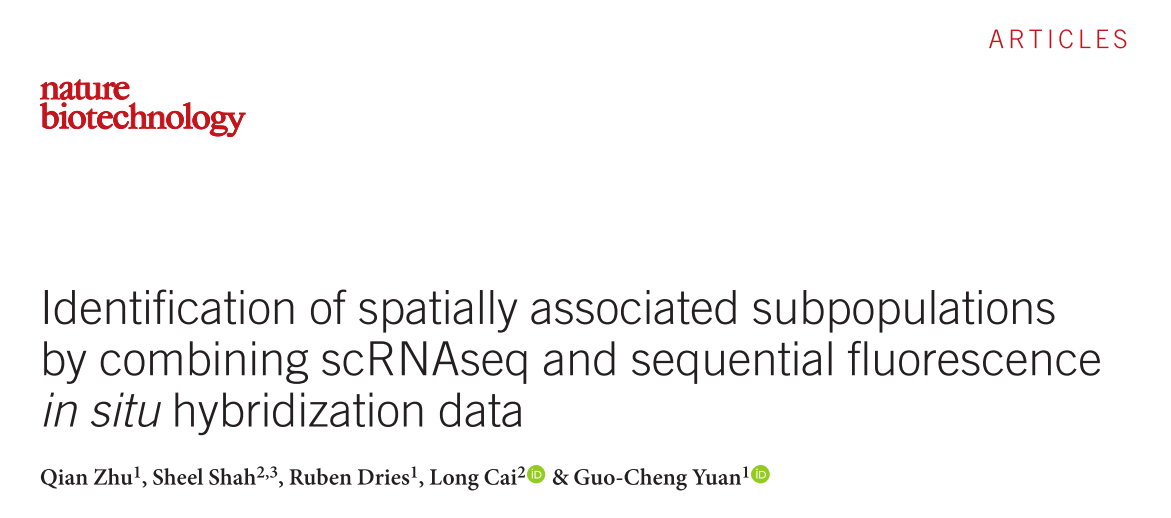
\includegraphics[width=\textwidth]{title}} % The short title appears at the bottom of every slide, the full title is only on the title page
\author{Faculty: Mengjie Chen \& Student: Yanyu Liang}
\institute[]
{
GGSB Journal Club
}
\date{5/2/19} % Date, can be changed to a custom date


\begin{document}

\begin{frame}
\titlepage % Print the title page as the first slide
\end{frame}
\addtocontents{toc}{\setcounter{tocdepth}{1}}
\begin{frame}
\frametitle{Overview} % Table of contents slide, comment this block out to remove it
\tableofcontents % Throughout your presentation, if you choose to use \section{} and \subsection{} commands, these will automatically be printed on this slide as an overview of your presentation
\end{frame}

%----------------------------------------------------------------------------------------
% PRESENTATION SLIDES
%----------------------------------------------------------------------------------------


%------------------------------------------------
\section{Background - On the other side of NGS}
%------------------------------------------------

  \begin{frame}
  \frametitle{FISH and single molecule FISH}
  \begin{figure}
    \centering
    \begin{minipage}{.5\textwidth}
        \centering
        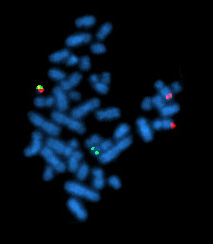
\includegraphics[width=0.45\linewidth]{Bcrablmet}
        \caption{FISH} \cite{wiki:Fluorescence_in_situ_hybridization}
    \end{minipage}%
    \begin{minipage}{0.5\textwidth}
        \centering
        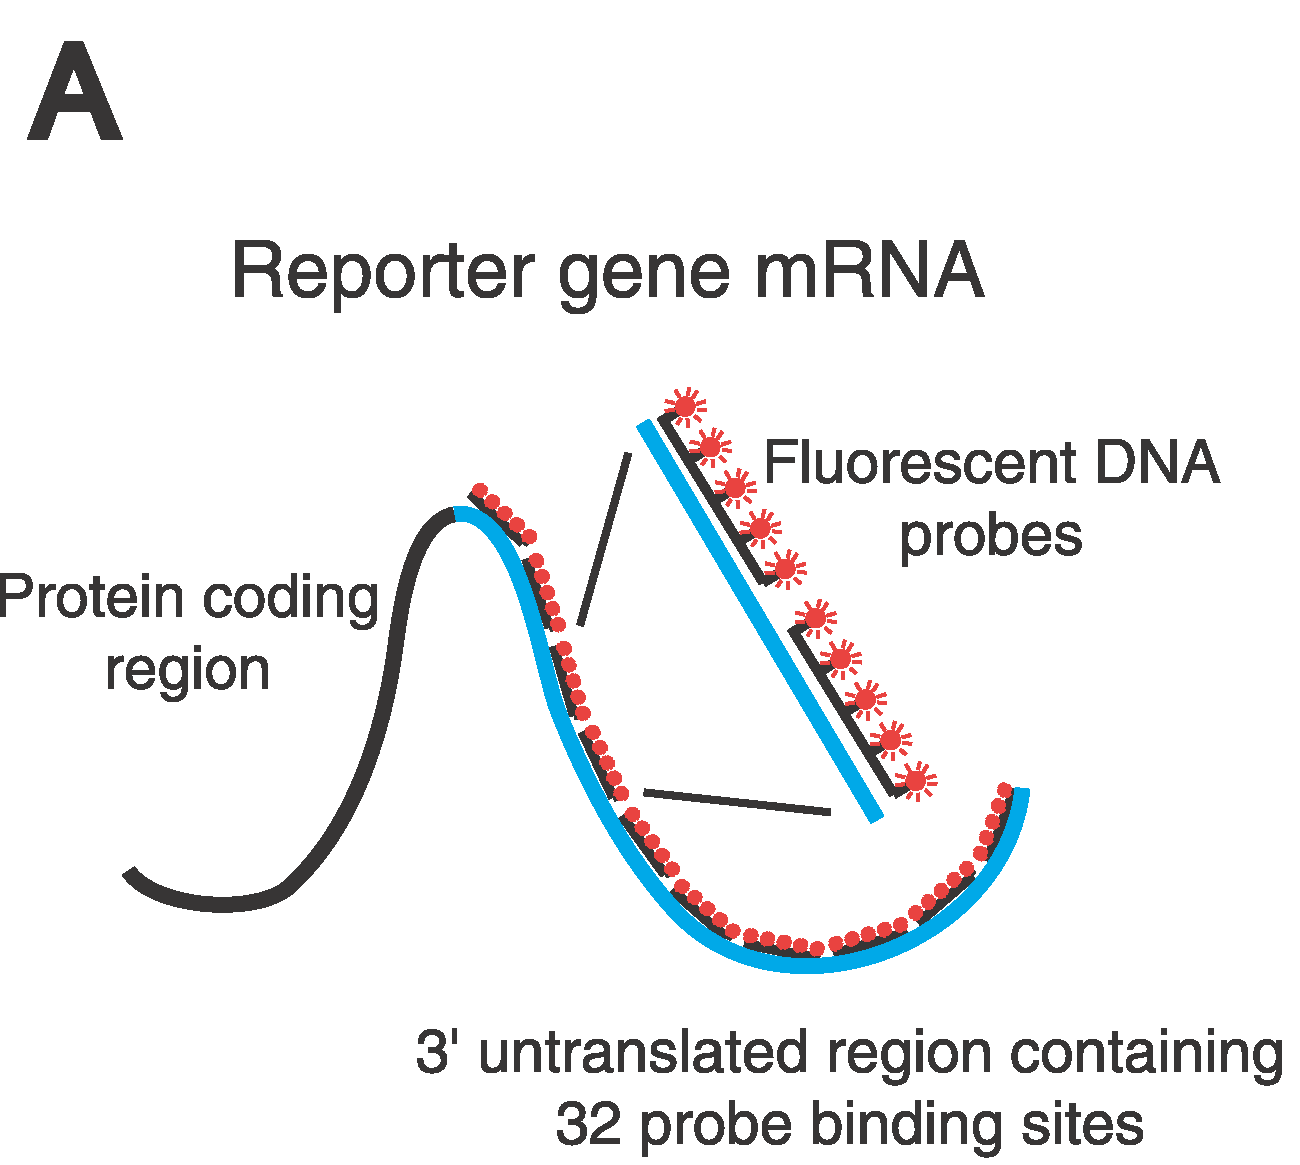
\includegraphics[width=0.6\linewidth]{smfish}
        \caption{smFISH} \cite{raj2006stochastic}
    \end{minipage}
  \end{figure}
  \begin{itemize}
    \item FISH: fluorescence in situ hybridization
    \item Single molecule FISH: pioneered by \cite{femino1998visualization}, enhanced version by \cite{raj2006stochastic}
      \begin{itemize}
        \item Multiple short probe/fluorophore $\rightarrow$ Brighter $\rightarrow$ Higher sensitivity and specificity
      \end{itemize}
  \end{itemize}
  \end{frame}

  \begin{frame}
  \frametitle{Super-resolution microscopy}
  \begin{figure}
    \centering
    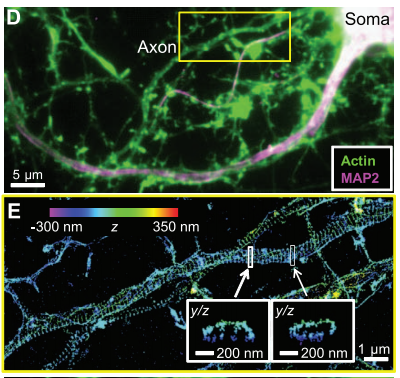
\includegraphics[width=0.4\textwidth]{storm}
    \caption{STORM image of neuron} \cite{xu2013actin}
  \end{figure}
  \begin{itemize}
    \item Resolution 10-20 nm on x, y and $<50$ nm on z direction.
    \item It helps to reveal finer structure (under diffraction barrier, $\sim 250$nm)
  \end{itemize}
  \end{frame}

  \begin{frame}
  \frametitle{Sequencing by hybridization}

  \begin{itemize}
    \item Encode sequence by combination of color \cite{lubeck2012single}
    \item Encode sequence by order of color \cite{lubeck2014single} (seqFISH)
    \item Two rounds three channels:
      \begin{itemize}
        \item \red - \cyan $\rightarrow$ Gene 1
        \item \green - \cyan $\rightarrow$ Gene 2
        \item \cyan - \red $\rightarrow$ Gene 3
      \end{itemize}
    \item The complexity of the target library: number of hybridization $\times$ number of channels/probes
  \end{itemize}
  \end{frame}

  \begin{frame}
  \frametitle{Sequential FISH: an example}
  \begin{figure}
    \centering
    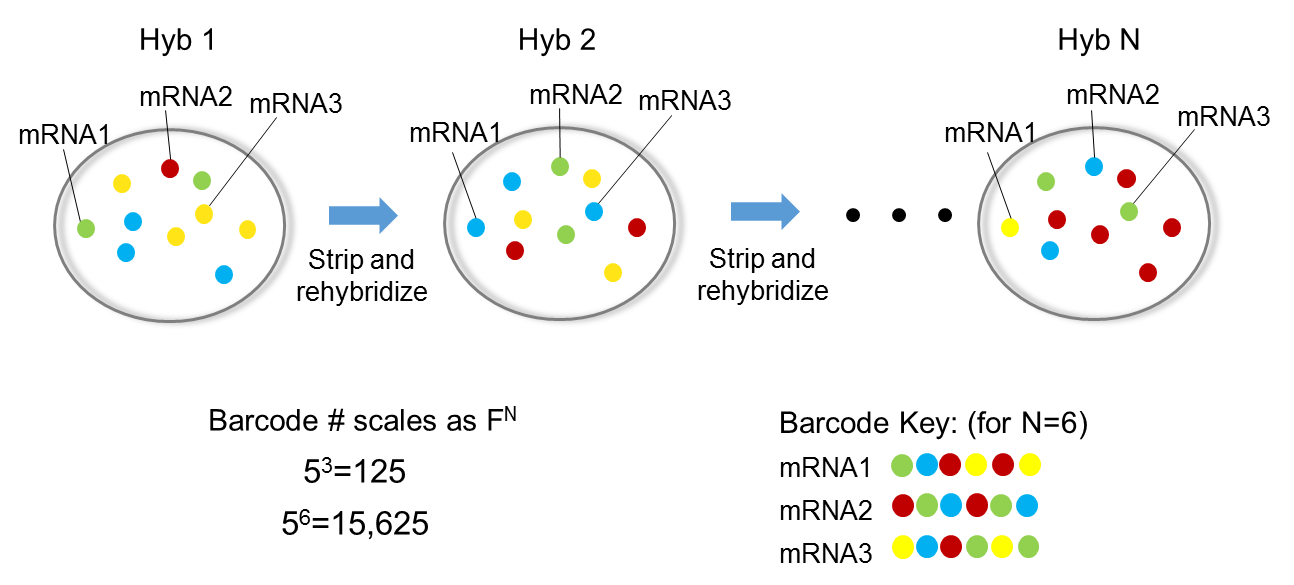
\includegraphics[width=0.8\textwidth]{seqFISH-Barcoding}
    \caption{seqFISH barcoding: four colors 6 rounds} \cite{seqfish}
  \end{figure}
  \end{frame}

  \begin{frame}
  \frametitle{What is good about seqFISH?}
  \begin{itemize}
    \item Low drop out rate ($\sim 94\%$ per round) \cite{shah2016situ}
    \item So that it is also easy to correct for this drop out error by one extra round
    \item As an in situ technology, it preserves spatial information which is erased in scRNA-seq
  \end{itemize}
  \end{frame}

%------------------------------------------------
\section{Main - Paper discussion}
%------------------------------------------------

  \begin{frame}
  \frametitle{Bring spatial information into scRNAseq}
  \begin{columns}
  \begin{column}{0.5\textwidth}
    \begin{itemize}
      \item Sources of variation in gene expression:
      \begin{itemize}
        \item Cell type?
        \item Cell state?
        \item Cell cycle?
        \item Spatial localization?
      \end{itemize}
      \item Benefit: account for spatial variation in differential analysis
    \end{itemize}
  \end{column}
  \begin{column}{0.5\textwidth}  %%<--- here
    \begin{figure}
      \centering
      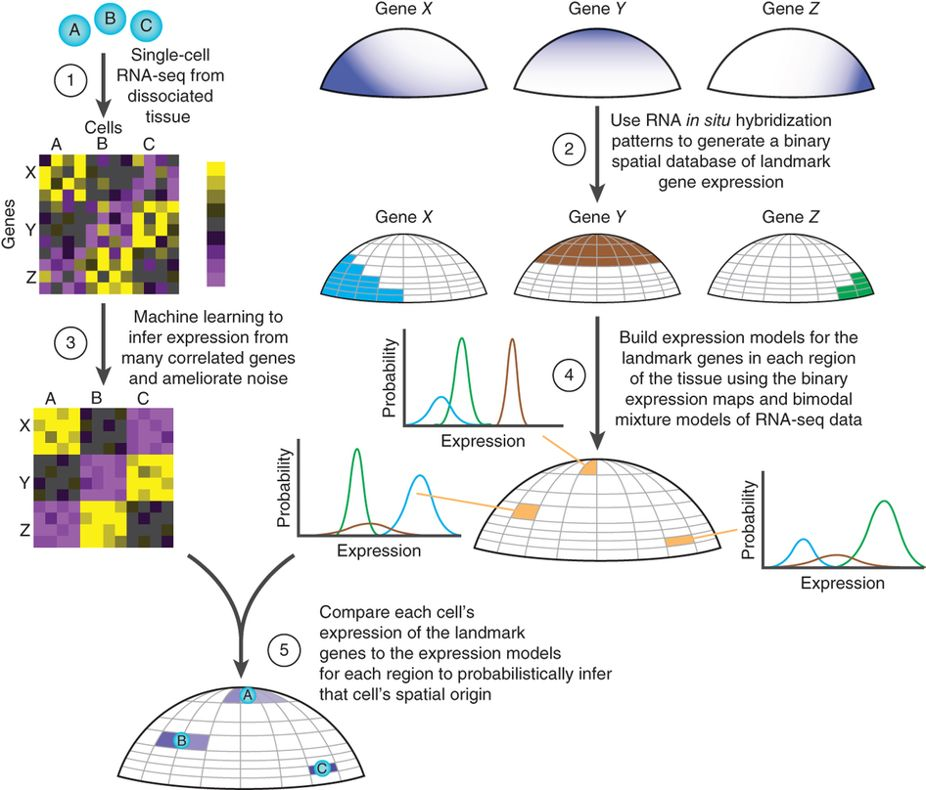
\includegraphics[width=0.9\textwidth]{seurat}
      \caption{An example: using spatial marker genes in embryo} \cite{Satija2015}
    \end{figure}
  \end{column}
  \end{columns}
  \end{frame}

  \begin{frame}
  \frametitle{Combine seqFISH and scRNAseq}
  \begin{figure}
    \centering
    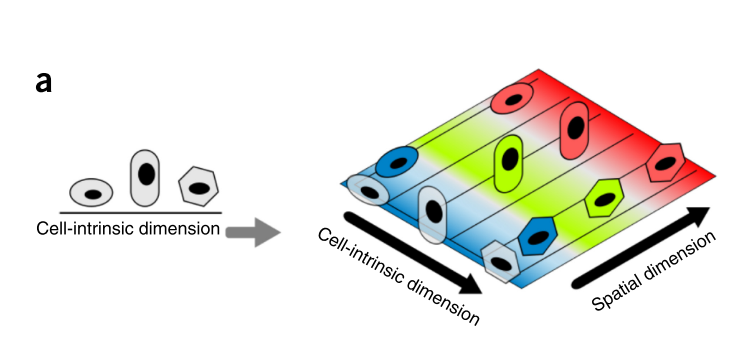
\includegraphics[width=0.6\textwidth]{variation} (fig1a)
  \end{figure}
  \begin{columns}
  \begin{column}{0.5\textwidth}
    \textbf{Several questions}:
    \begin{itemize}
      \item Is there any spatial pattern/variation in gene expression profile?
      \item How to quantify/account for spatial variation if it exists?
      \item What do we learn about spatial variation?
    \end{itemize}
  \end{column}
  \begin{column}{0.5\textwidth}  %%<--- here
    \textbf{In this paper}:
    \begin{itemize}
      \item Detect spatial pattern using HMRF
      \item Construct a set of spatial markers
      \item Within cell type, how spatial difference contributes to heterogeneity
    \end{itemize}
  \end{column}
  \end{columns}
  \end{frame}

  \begin{frame}
  \frametitle{Collect seqFISH and scRNAseq data}
  \begin{figure}
    \centering
    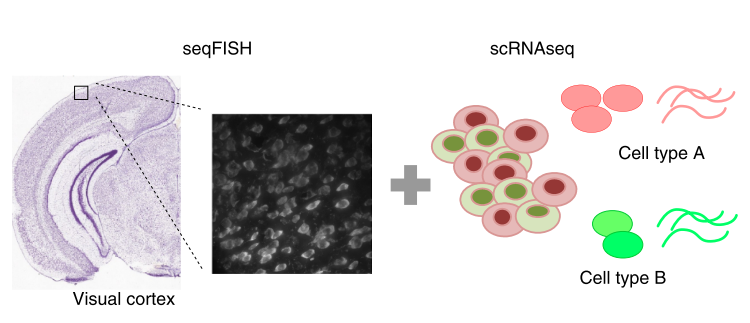
\includegraphics[width=0.7\textwidth]{data} (fig1b)
  \end{figure}
  \begin{columns}
  \begin{column}{0.4\textwidth}
    \textbf{seqFISH}:
    \begin{itemize}
      \item 1-mm $\times$ 1-mm contiguous area of the mouse visual cortex
      \item 5 colors, 4 rounds
      \item 125 genes were profiled in 1597 cells
    \end{itemize}
  \end{column}
  \begin{column}{0.6\textwidth}  %%<--- here
    \textbf{scRNAseq}:
    \begin{itemize}
      \item Published scRNAseq data set on the mouse visual cortex region
      \item 8 major cell types identified: GABAergic, glutamatergic, astrocytes, three oligodendrocyte groups, microglia and endothelial cells
    \end{itemize}
  \end{column}
  \end{columns}
  \end{frame}

  \begin{frame}
  \frametitle{Identify spatial pattern}
  \begin{itemize}
    \item Spatial pattern of interest:
    \begin{itemize}
      \item Sub-region with region-specific expression profile
        % $$\Pr(\text{expression profile of cell }i | \text{region assignment of cell }i)$$
      \item Nearby cells are likely to be in the same sub-region
        % $$\Pr(\text{region assignment of cell }i | \text{region assignment of neighbours of cell} i)$$
    \end{itemize}
    \item Data with such spatial pattern can be easily described by hidden Markov random field (HMRF)
    \begin{itemize}
      \item $C_i$ region assignment of cell $i$
      \item $E_i$ expression profile of cell $i$
      \item Markov random field
        $$\Pr(C_i | \text{neighbours of } C_i)$$
      \item Expression profile signature for each sub-region
        $$\Pr(E_i | C_i)$$
    \end{itemize}
  \end{itemize}
  \end{frame}

  \begin{frame}
  \frametitle{Hidden Markov random field}
  \begin{figure}
    \centering
    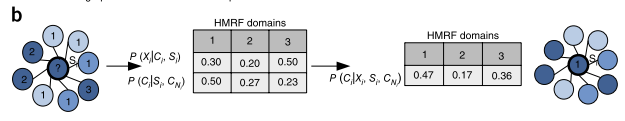
\includegraphics[width=0.7\textwidth]{mrf} (fig2b)
  \end{figure}
  \begin{figure}
    \centering
    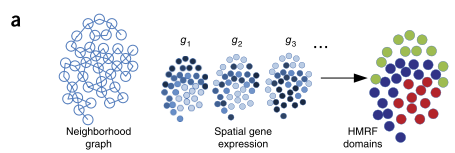
\includegraphics[width=0.7\textwidth]{hmrf} (fig2a)
  \end{figure}
  \end{frame}

  \begin{frame}
  \frametitle{Apply to seqFISH data}
  \begin{itemize}
    \item Pre-select a set of genes with spatial coherence (similar if spatially close), \cref{sec:sup1}
    \item Determine the neighbours of a cell by spatial information captured by seqFISH
    \item Fit HMRF by EM algorithm (determine the number of sub-regions by Kmeans, \cref{sec:sup2})
  \end{itemize}
  \end{frame}

  \begin{frame}
  \frametitle{Spatial dissection of seqFISH data}
  \begin{figure}
    \centering
    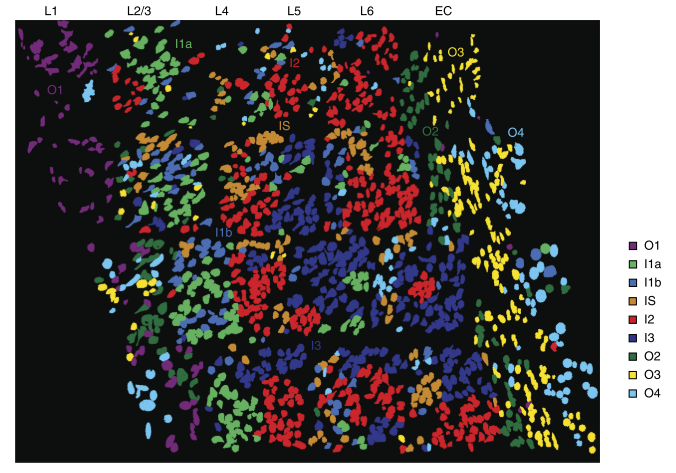
\includegraphics[width=0.7\textwidth]{subregion} (fig2c)
  \end{figure}
  \begin{itemize}
    \item 69 out of 125 genes were used
    \item 9 sub-regions identified
    \item Resembled anatomical structure
  \end{itemize}
  \end{frame}

  \begin{frame}
  \frametitle{Identify region-specific genes}
  \begin{columns}
  \begin{column}{0.4\textwidth}
    For each sub-region, if a gene is
    \begin{itemize}
      \item Significantly up-regulated as compared to 7 out of 8 other sub-region
      \item Significantly up-regulated as compared to all the rest (p-value shown on the right)
    \end{itemize}
    The gene is identified as domain signature
  \end{column}
  \begin{column}{0.6\textwidth}  %%<--- here
    \begin{figure}
      \centering
      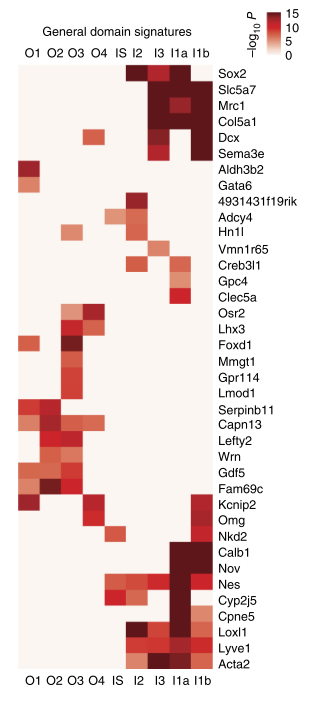
\includegraphics[width=0.5\textwidth]{sig_gene} (fig2d)
    \end{figure}
  \end{column}
  \end{columns}
  \end{frame}

  \begin{frame}
  \frametitle{Impute cell type?}
  \begin{itemize}
    \item Use scRNAseq data to learn the charateristics of each cell type
    \item Since genes are highly correlated, using $\sim$ 40 genes have already give 89\% accuracy
    \item Match the scale of scRNAseq and seqFISH by quantile normalization
  \end{itemize}
  \end{frame}

  \begin{frame}
  \frametitle{Impute cell type in seqFISH using scRNAseq}
  \begin{columns}
  \begin{column}{0.5\textwidth}
    \begin{itemize}
      \item 43 out of 125 differentially expressed seqFISH genes were used achieving 90\% accuracy on scRNAseq
      \item 1597 seqFISH cells were classified into: glutamatergic neurons (54\%), GABAergic neurons (37\%), astrocytes (4.8\%), and other glial cell types and endothelial cells (4.2\%)
    \end{itemize}
  \end{column}
  \begin{column}{0.5\textwidth}  %%<--- here
    \begin{figure}
      \centering
      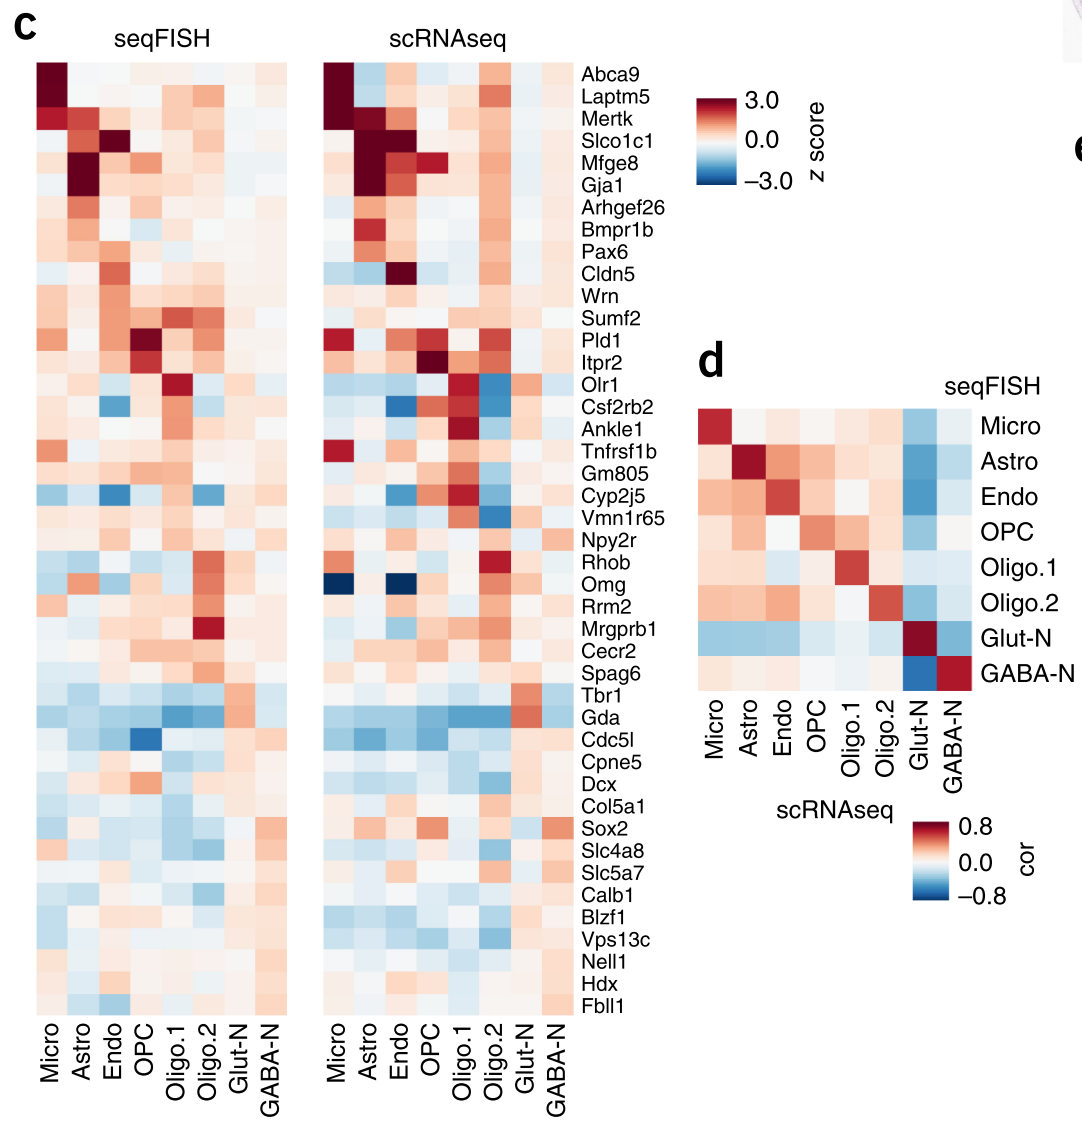
\includegraphics[width=0.95\textwidth]{cell_type_gene} (fig1c,d)
    \end{figure}
  \end{column}
  \end{columns}
  \end{frame}

  \begin{frame}
  \frametitle{Spatial distribution of cell type}
  \begin{figure}
    \centering
    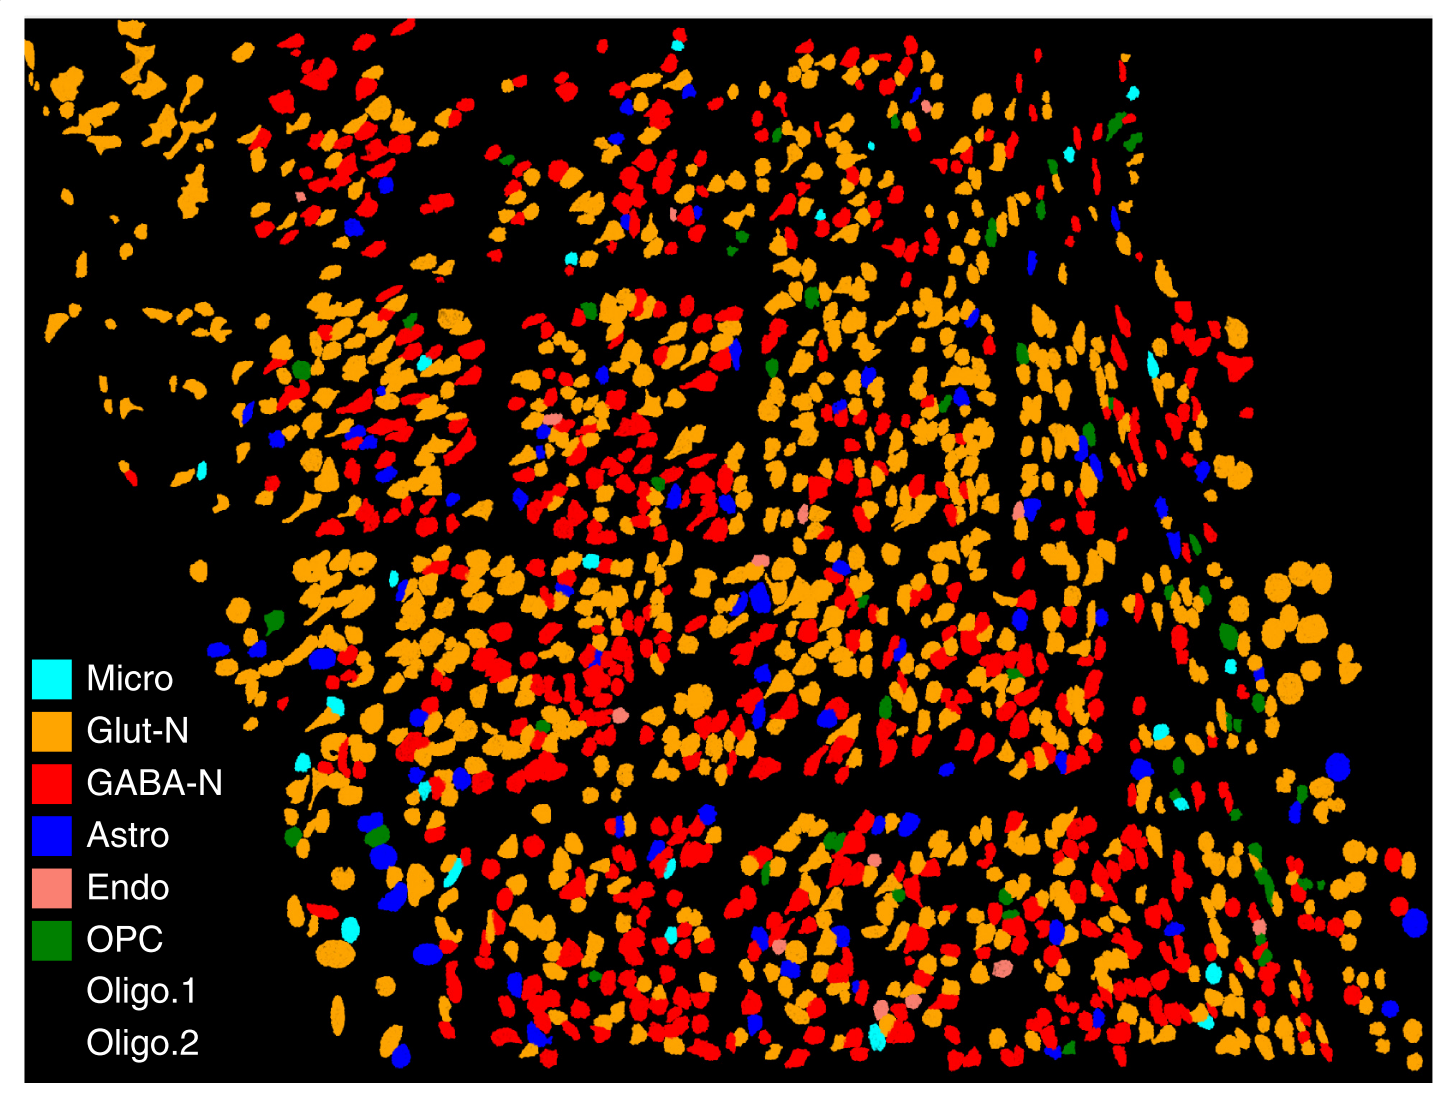
\includegraphics[width=0.8\textwidth]{cell_type} (fig1e)
    \caption{In glutamatergic cells}
  \end{figure}
  \end{frame}

  \begin{frame}
  \frametitle{How does spatial variation contribute to cellular heterogeneity?}
  \begin{figure}
    \centering
    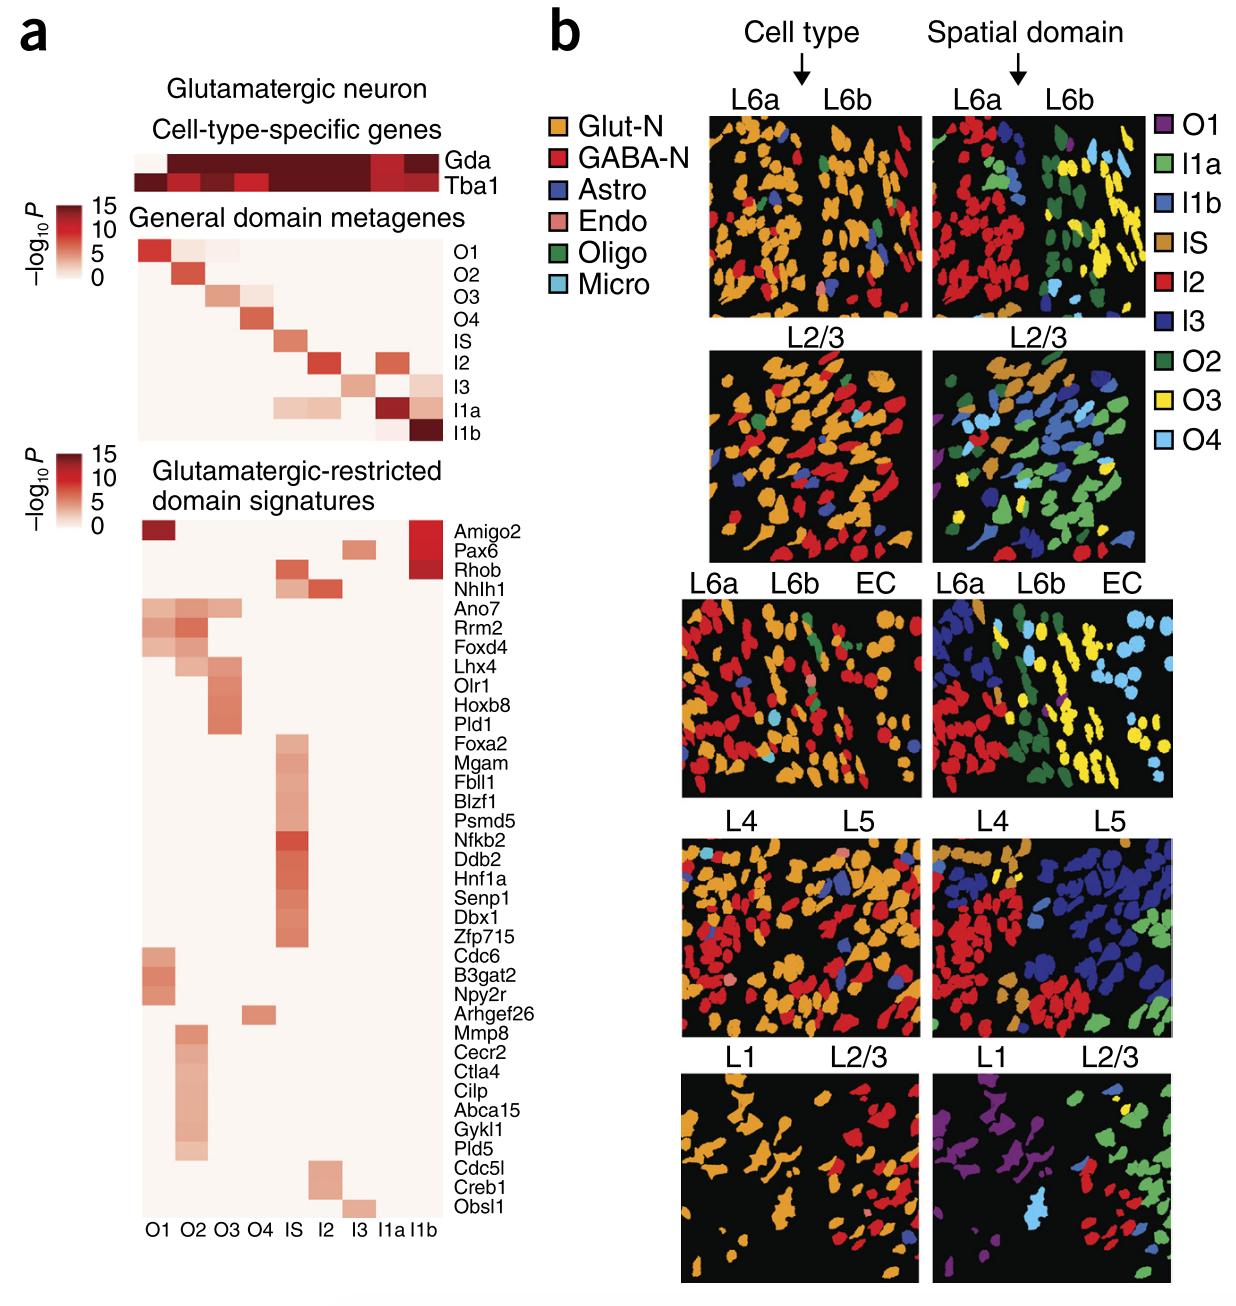
\includegraphics[width=0.6\textwidth]{heter} (fig3)
  \end{figure}
  \end{frame}

  \begin{frame}
  \frametitle{Re-analyze scRNAseq with imputed spatial assignment: spatial pattern}
  \begin{columns}
  \begin{column}{0.5\textwidth}
    \begin{figure}
      \centering
      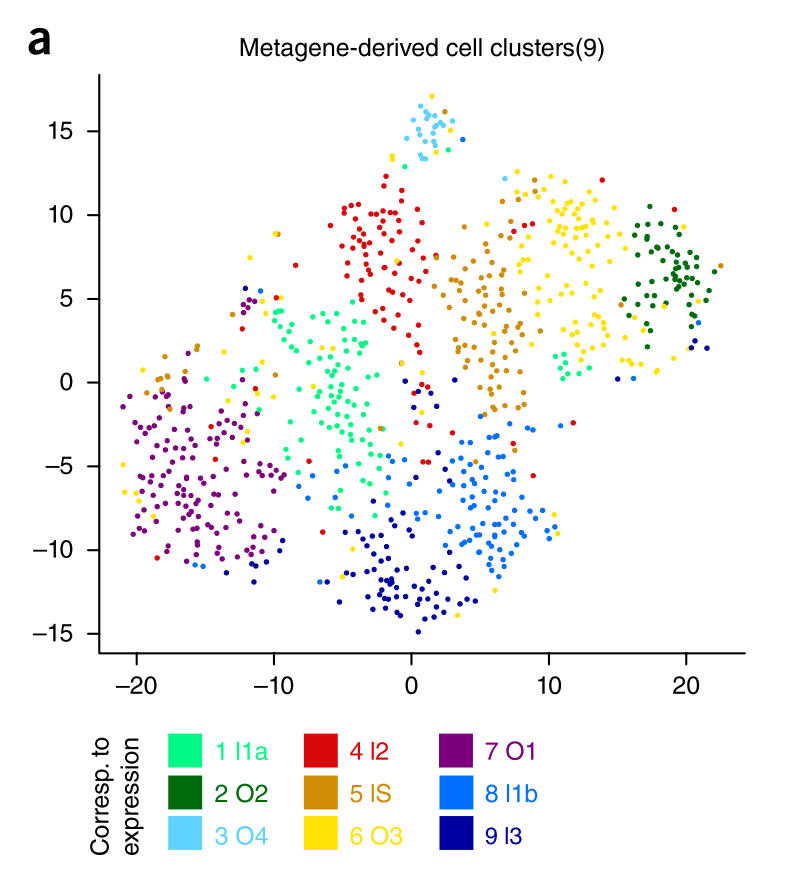
\includegraphics[width=0.9\textwidth]{glu_tsne} (fig4a)
    \end{figure}
  \end{column}
  \begin{column}{0.5\textwidth}
    \begin{figure}
      \centering
      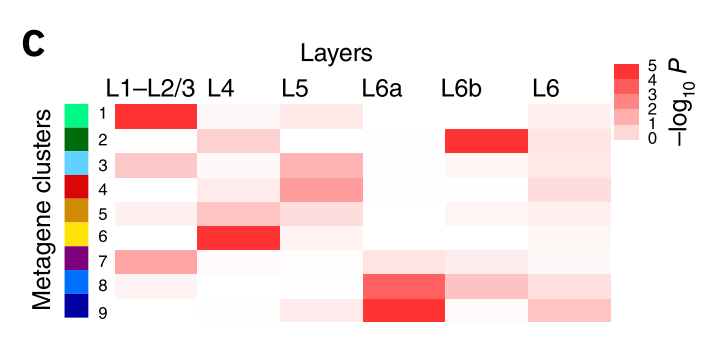
\includegraphics[width=0.9\textwidth]{glu_ana} (fig4c)
    \end{figure}
    Spatial pattern also appears in scRNAseq data
  \end{column}
  \end{columns}
  \end{frame}

  \begin{frame}
  \frametitle{Re-analyze scRNAseq with imputed spatial assignment: spatial markers}
  With enlarged gene sets, more domain-specific genes were identified. And they are enriched in distinct Gene Ontology biological processes
  \begin{figure}
    \centering
    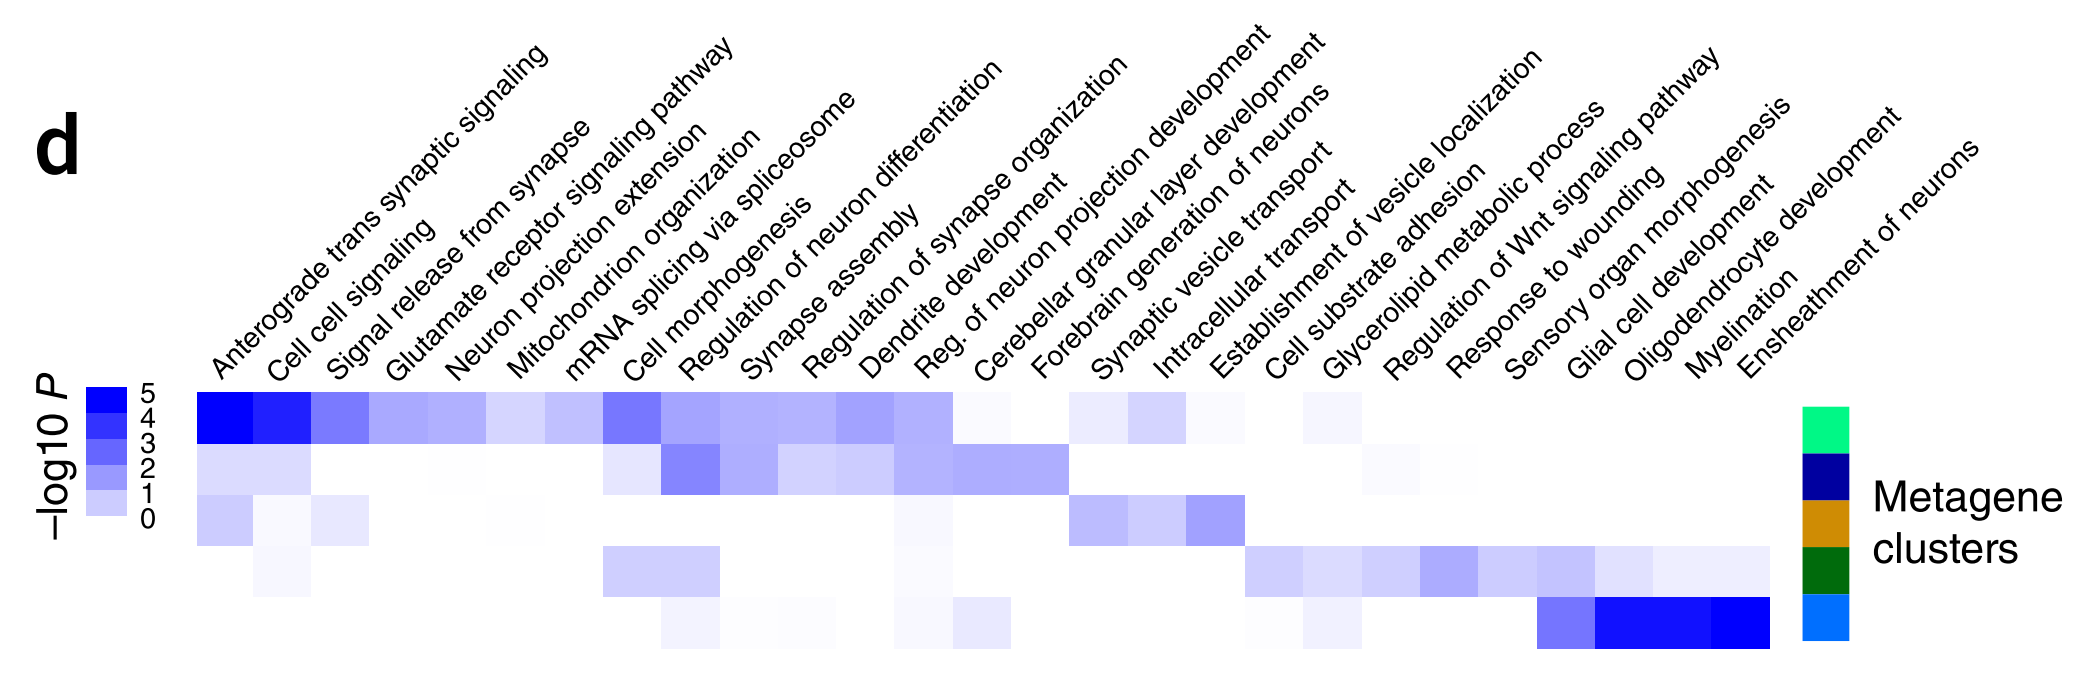
\includegraphics[width=0.9\textwidth]{enrich} (fig4d)
  \end{figure}
  \end{frame}

  \begin{frame}
  \frametitle{Does spatial variation explain cell subtypes?}
  \begin{figure}
    \centering
    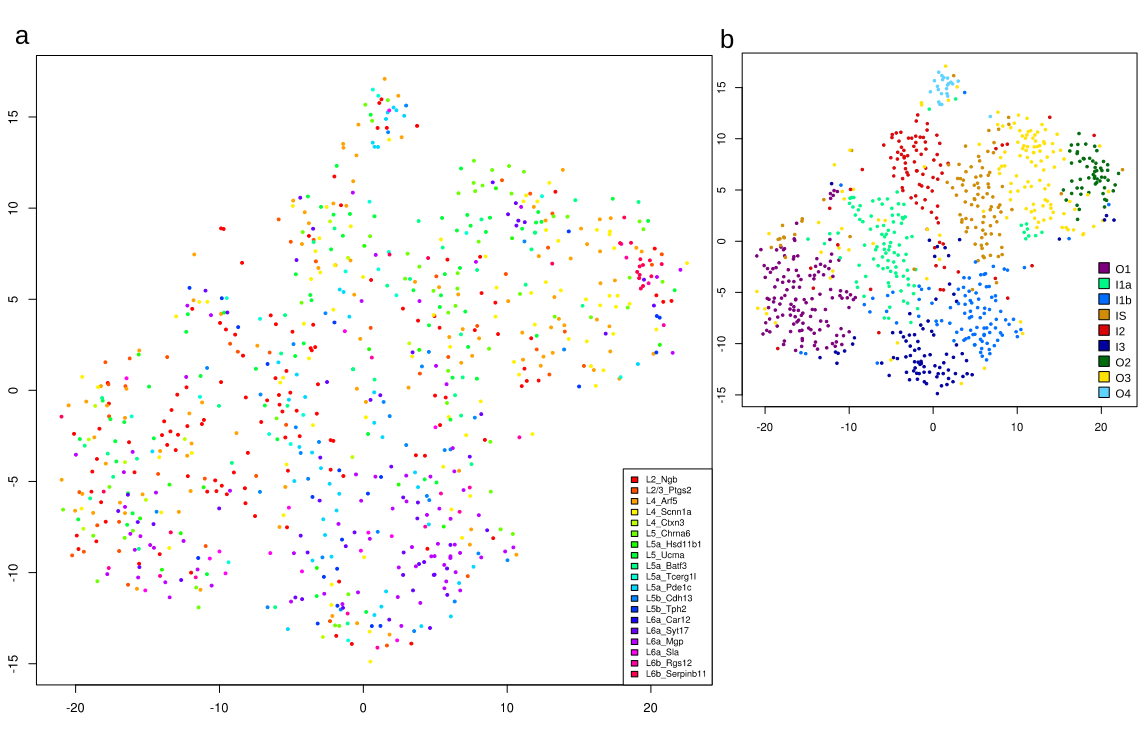
\includegraphics[width=0.9\textwidth]{subtype} (figS14)
  \end{figure}
  \end{frame}

  \begin{frame}
  \frametitle{Take-aways}
  \begin{itemize}
    \item There is clear spatial pattern in visual cortex of mouse
    \item Such spatial variation contributes to heterogeneity of cells (expression and morphology)
    \item And it is distinct source variation as compared to cell subtype (based on expression profile)
  \end{itemize}
  \end{frame}

%------------------------------------------------
\section{Spatial genomics - what else?}
%------------------------------------------------

  \begin{frame}
  \frametitle{Technology side - expansion microscopy}
  \begin{figure}
    \centering
    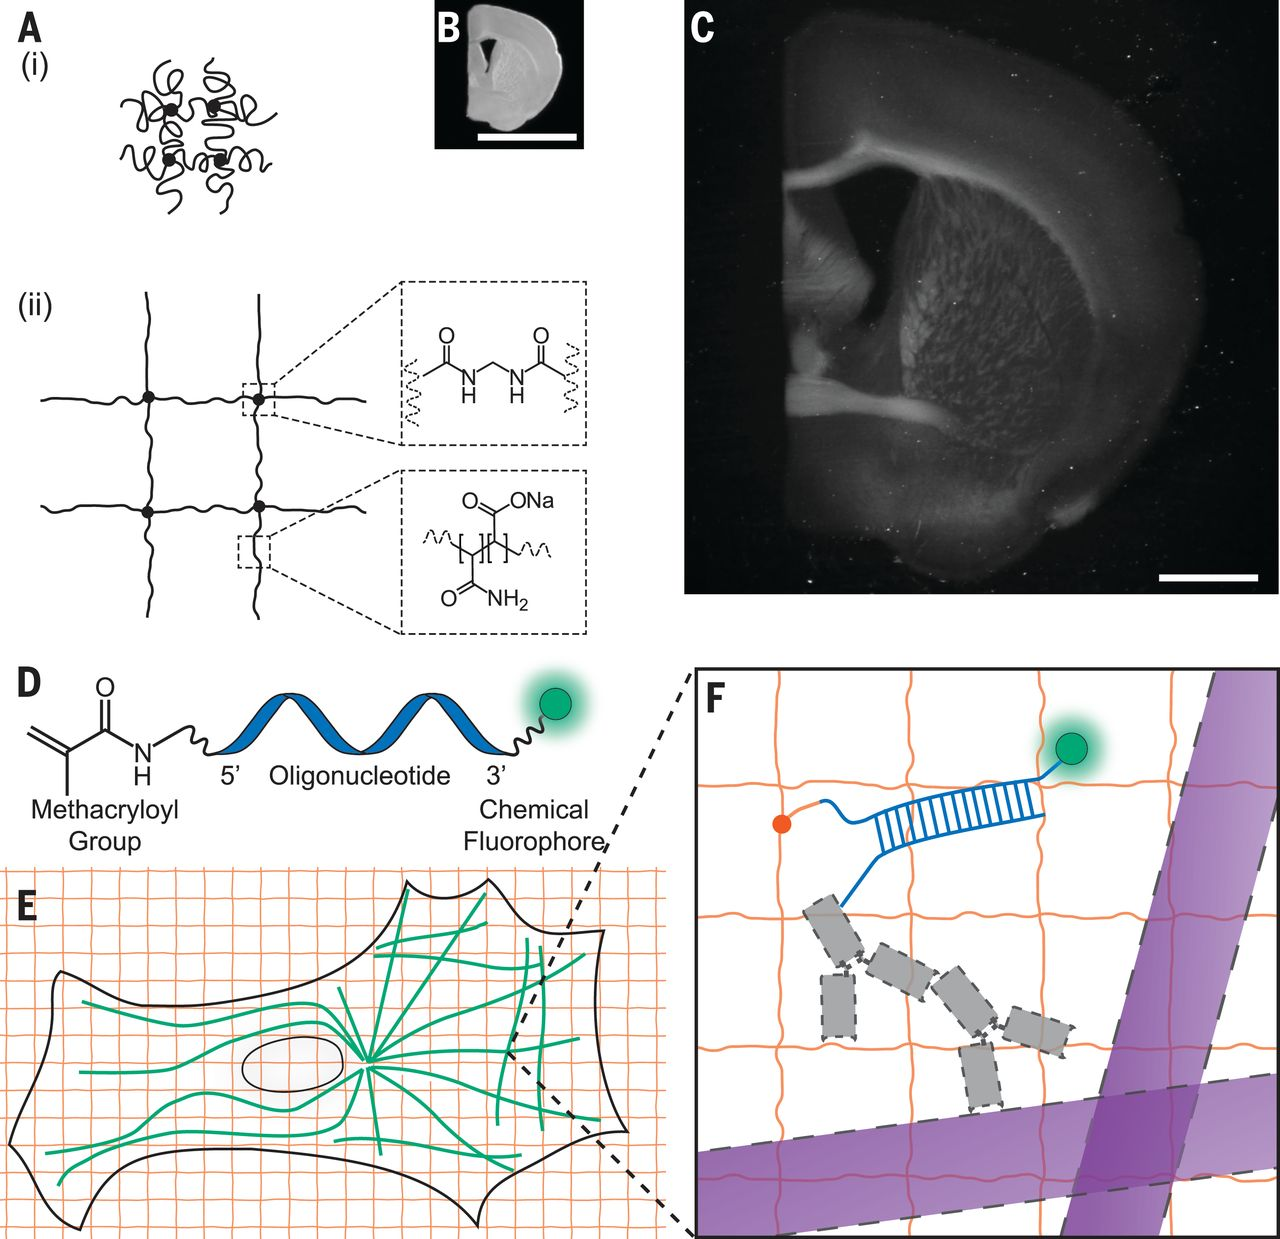
\includegraphics[width=0.6\textwidth]{expansion}
    \cite{chen2015expansion}
  \end{figure}
  Fixing molecule on gel and expand gel so that the object of interest is enlarged isotropically.
  \end{frame}

  \begin{frame}
  \frametitle{Technology side - SeqFISH+}
  \begin{figure}
    \centering
    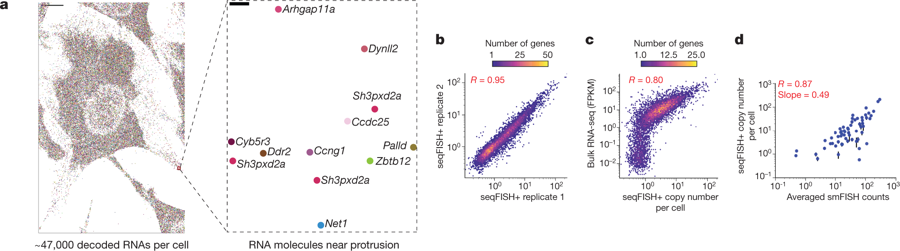
\includegraphics[width=\textwidth]{seqfishp}
    \cite{eng2019transcriptome}
  \end{figure}
  \begin{itemize}
    \item Dilute signal by 60 psuedo-colors (in three channels); 3 rounds plus one for error correction ($\underbrace{20^3}_{\text{each channel}} \times \underbrace{3}_{\text{number of channels}}$)
    \item 10000 genes, $\sim$ 3000 cells, efficacy 49\% (compared to smFISH)
  \end{itemize}
  \end{frame}

  \begin{frame}
  \frametitle{Application side - chromatin interaction}
  \begin{figure}
    \centering
    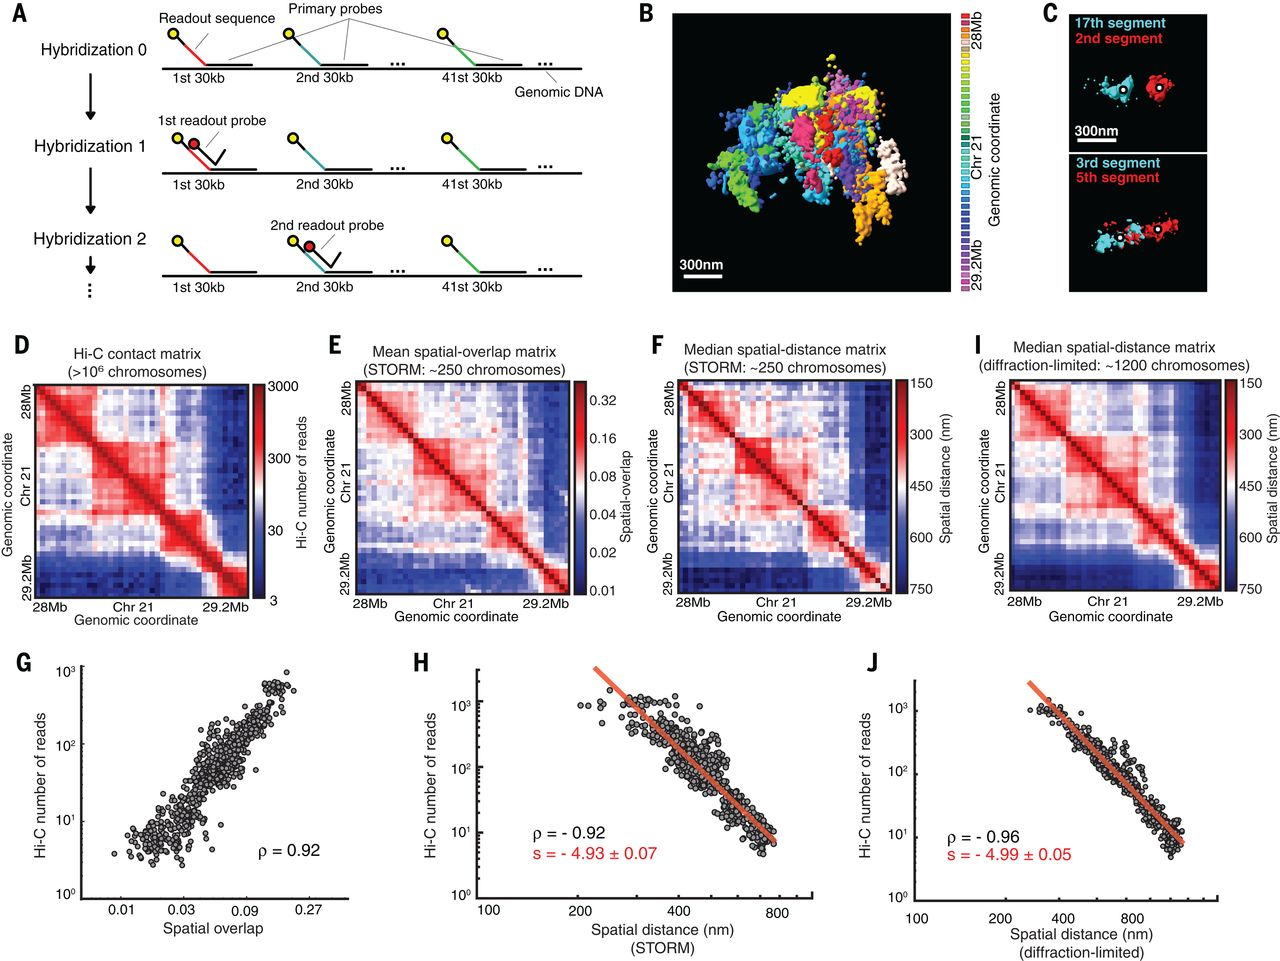
\includegraphics[width=0.6\textwidth]{chromatin}
    \cite{bintu2018super}
  \end{figure}
  \begin{itemize}
    \item Sequence resolution in kb, spatial resolution in nanometer, profiled thousands of single cells
    \item Recover Hi-C result by population averaging
    \item BUT with single cell resolution and higher-order interaction
  \end{itemize}
  \end{frame}

  \begin{frame}
  \frametitle{Application side - beyond mRNA}
  \begin{figure}
    \centering
    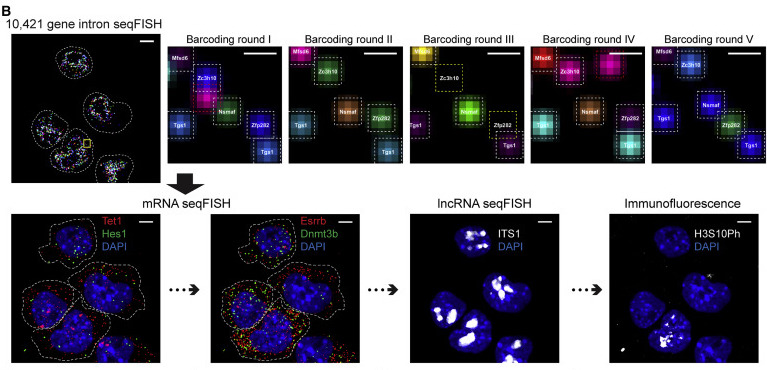
\includegraphics[width=0.8\textwidth]{gr1}
    \cite{shah2018dynamics}
  \end{figure}
  \begin{itemize}
    \item Nascent transcriptome with mRNAs and lncRNAs profiled in the same cell
  \end{itemize}
  \end{frame}

  \begin{frame}
  \frametitle{Application side - imaging allele-specific expression}
  \begin{figure}
    \centering
    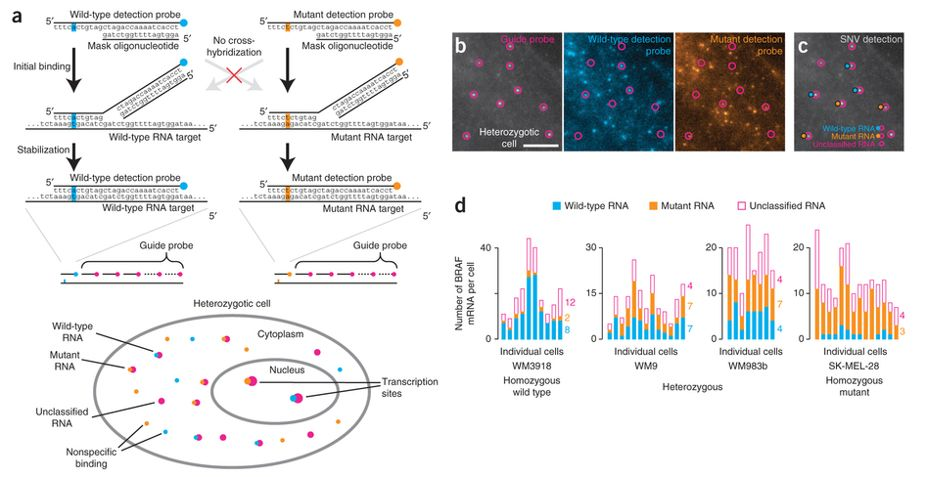
\includegraphics[width=0.8\textwidth]{ase}
    \cite{levesque2013visualizing}
  \end{figure}
  \begin{itemize}
    \item Clever design on probe to enable allele-specific detection
  \end{itemize}
  \end{frame}

  \begin{frame}
  \frametitle{Any downside? Of course}
  \begin{itemize}
    \item Protocol is hard to implement ...
    \item To image real-world sample can be very challenging (transparency, thickness)
    \item Lack of isoform information (although it is possible)
  \end{itemize}
  \end{frame}

\begin{frame}{}
  \centering \Huge
  \emph{Thank You}
\end{frame}

%------------------------------------------------
\begin{frame}[allowframebreaks]
\frametitle{References}
\footnotesize
\bibliography{ref}
\bibliographystyle{apalike}
\end{frame}
%----------------------------------------------------------------------------------------

\appendix
\section{Supplements}

\begin{frame}[label=supplemental] \label{sec:sup1}
Coherent score: $\delta_g = \frac{1}{|L_1|} \sum_{s_i \in L_1} \frac{m_i - n_i}{\max(m_i, n_i)}$, $L_1$ highly expressed cells, $m_i$ average 'distance' to $L_0$, $n_i$ average 'distance' to $L_1$. Significance of $\delta_g$ is done by permutation.
\end{frame}

\begin{frame}[label=supplemental] \label{sec:sup2}
Select the number of clusters: gap statistic, $gap(k) = \mathbb{E}[\log W_k] - \log W_k$, $W_k$ is the sum of average within cluster squared distance. Expectation is taken under the null (no cluster structure; obtained from Bootstrap). Criteria: smallest $k$ such that $gap(k+1) - sd(k+1) < gap(k)$ (namely no significant increase). Select $k$ by gap statistic under k-means
\end{frame}

%----------------------------------------------------------------------------------------



\end{document}
